\documentclass[a4paper, final]{article}
%\usepackage{literat} % Нормальные шрифты
\usepackage[12pt]{extsizes} % для того чтобы задать нестандартный 14-ый размер шрифта
\usepackage{tabularx}
\usepackage[T2A]{fontenc}
\usepackage[utf8]{inputenc}
\usepackage[russian]{babel}
\usepackage{amsmath}
\usepackage[left=25mm, top=20mm, right=20mm, bottom=20mm, footskip=10mm]{geometry}
\usepackage{ragged2e} %для растягивания по ширине
\usepackage{setspace} %для межстрочного интервала
\usepackage{moreverb} %для работы с листингами
\usepackage{indentfirst} % для абзацного отступа
\usepackage{moreverb} %для печати в листинге исходного кода программ
\usepackage{pdfpages} %для вставки других pdf файлов
\usepackage{tikz}
\usepackage{graphicx}
\usepackage{afterpage}
\usepackage{longtable}
\usepackage{float}



% \usepackage[paper=A4,DIV=12]{typearea}
\usepackage{pdflscape}
% \usepackage{lscape}

\usepackage{array}
\usepackage{multirow}

\renewcommand\verbatimtabsize{4\relax}
\renewcommand\listingoffset{0.2em} %отступ от номеров строк в листинге
\renewcommand{\arraystretch}{1.4} % изменяю высоту строки в таблице
\usepackage[font=small, singlelinecheck=false, justification=centering, format=plain, labelsep=period]{caption} %для настройки заголовка таблицы
\usepackage{listings} %листинги
\usepackage{xcolor} % цвета
\usepackage{hyperref}% для гиперссылок
\usepackage{enumitem} %для перечислений

% Настраиваем листинги, чтобы они использовали счётчик figure
% \AtBeginDocument{
%   \renewcommand{\thelstlisting}{\thefigure}  % Листинги используют тот же счетчик, что и рисунки
%   \renewcommand{\lstlistingname}{Рис.}    % Меняем подпись на "Рисунок"
% }

% Автоматически увеличиваем счетчик figure перед каждым листингом
% \let\oldlstlisting\lstlisting
% \renewcommand{\lstlisting}[1][]{%
%     \refstepcounter{figure}% Увеличиваем счетчик figure
%     \oldlstlisting[#1]% Вызываем оригинальную команду lstlisting
% }

\newcommand{\specialcell}[2][l]{\begin{tabular}[#1]{@{}l@{}}#2\end{tabular}}


\setlist[enumerate,itemize]{leftmargin=1.2cm} %отступ в перечислениях

\hypersetup{colorlinks,
allcolors=[RGB]{010 090 200}} %красивые гиперссылки (не красные)

% подгружаемые языки — подробнее в документации listings (это всё для листингов)
\lstloadlanguages{ Haskell}
% включаем кириллицу и добавляем кое−какие опции
\lstset{tabsize=2,
breaklines,
basicstyle=\footnotesize,
columns=fullflexible,
flexiblecolumns,
numbers=left,
numberstyle={\footnotesize},
keywordstyle=\color{blue},
inputencoding=cp1251,
extendedchars=true
}
\lstdefinelanguage{MyC}{
language=Haskell,
%    ndkeywordstyle=\color{darkgray}\bfseries,
%    identifierstyle=\color{black},
%    morecomment=[n]{/**}{*/},
%    commentstyle=\color{blue}\ttfamily,
%    stringstyle=\color{red}\ttfamily,
%    morestring=[b]",
%    showstringspaces=false,
%    morecomment=[l][\color{gray}]{//},
keepspaces=true,
escapechar=\%,
texcl=true
}

\textheight=24cm % высота текста
\textwidth=16cm % ширина текста
\oddsidemargin=0pt % отступ от левого края
\topmargin=-1.5cm % отступ от верхнего края
\parindent=24pt % абзацный отступ
\parskip=5pt % интервал между абзацами
\tolerance=2000 % терпимость к "жидким" строкам
\flushbottom % выравнивание высоты страниц


\lstset{
	backgroundcolor=\color{white},  % Устанавливаем белый фон для блока кода
	basicstyle=\ttfamily\small\fontfamily{inconsolata}\selectfont,  % Основной стиль текста: моноширинный шрифт Inconsolata с небольшим размером
	commentstyle=\color{darkgreen}\slshape,  % Комментарии будут зелеными и курсивными
	keywordstyle=\color{blue}\bfseries,  % Ключевые слова выделяются синим цветом и полужирным шрифтом
	numberstyle=\scriptsize\color{gray},  % Стиль нумерации строк: маленький размер шрифта и серый цвет
	stringstyle=\color{orange},  % Строки (текст в кавычках) отображаются оранжевым цветом
	breakatwhitespace=false,  % Не прерывать строки только по пробелам
	breaklines=true,  % Автоматический перенос длинных строк
	postbreak=\mbox{\textcolor{gray}{$\hookrightarrow$}}, % Символ переноса строки
	captionpos=b,  % Позиция заголовка/описания для блока кода — внизу (b — bottom)
	keepspaces=true,  % Сохранить пробелы, как они есть, в исходном коде
	numbers=left,  % Нумерация строк будет отображаться слева
	numbersep=5pt,  % Отступ между строками кода и номерами строк (4pt)
	showspaces=false,  % Не показывать пробелы
	showstringspaces=false,  % Не показывать пробелы внутри строк
	showtabs=false,  % Не показывать символы табуляции
	tabsize=4,  % Размер табуляции — 4 пробела
	language=Haskell,  % Указываем язык программирования для синтаксического подсветки (C++)
	captionpos=t,  % Заголовок кода будет размещен вверху (t — top)
	xleftmargin=0mm,  % Убираем отступ слева
	frame=single,  % Однотонная рамка вокруг блока кода
	framerule=0.25mm,  % Толщина рамки — 0.25 мм
	literate=
	{а}{{\selectfont\char224}}1
	{б}{{\selectfont\char225}}1
	{в}{{\selectfont\char226}}1
	{г}{{\selectfont\char227}}1
	{д}{{\selectfont\char228}}1
	{е}{{\selectfont\char229}}1
	{ж}{{\selectfont\char230}}1
	{з}{{\selectfont\char231}}1
	{и}{{\selectfont\char232}}1
	{й}{{\selectfont\char233}}1
	{к}{{\selectfont\char234}}1
	{л}{{\selectfont\char235}}1
	{м}{{\selectfont\char236}}1
	{н}{{\selectfont\char237}}1
	{о}{{\selectfont\char238}}1
	{п}{{\selectfont\char239}}1
	{р}{{\selectfont\char240}}1
	{с}{{\selectfont\char241}}1
	{т}{{\selectfont\char242}}1
	{у}{{\selectfont\char243}}1
	{ф}{{\selectfont\char244}}1
	{х}{{\selectfont\char245}}1
	{ц}{{\selectfont\char246}}1
	{ч}{{\selectfont\char247}}1
	{ш}{{\selectfont\char248}}1
	{щ}{{\selectfont\char249}}1
	{ъ}{{\selectfont\char250}}1
	{ы}{{\selectfont\char251}}1
	{ь}{{\selectfont\char252}}1
	{э}{{\selectfont\char253}}1
	{ю}{{\selectfont\char254}}1
	{я}{{\selectfont\char255}}1
	{А}{{\selectfont\char192}}1
	{Б}{{\selectfont\char193}}1
	{В}{{\selectfont\char194}}1
	{Г}{{\selectfont\char195}}1
	{Д}{{\selectfont\char196}}1
	{Е}{{\selectfont\char197}}1
	{Ж}{{\selectfont\char198}}1
	{З}{{\selectfont\char199}}1
	{И}{{\selectfont\char200}}1
	{Й}{{\selectfont\char201}}1
	{К}{{\selectfont\char202}}1
	{Л}{{\selectfont\char203}}1
	{М}{{\selectfont\char204}}1
	{Н}{{\selectfont\char205}}1
	{О}{{\selectfont\char206}}1
	{П}{{\selectfont\char207}}1
	{Р}{{\selectfont\char208}}1
	{С}{{\selectfont\char209}}1
	{Т}{{\selectfont\char210}}1
	{У}{{\selectfont\char211}}1
	{Ф}{{\selectfont\char212}}1
	{Х}{{\selectfont\char213}}1
	{Ц}{{\selectfont\char214}}1
	{Ч}{{\selectfont\char215}}1
	{Ш}{{\selectfont\char216}}1
	{Щ}{{\selectfont\char217}}1
	{Ъ}{{\selectfont\char218}}1
	{Ы}{{\selectfont\char219}}1
	{Ь}{{\selectfont\char220}}1
	{Э}{{\selectfont\char221}}1
	{Ю}{{\selectfont\char222}}1
	{Я}{{\selectfont\char223}}1,
	numbers=left, % пронумеровать строки с левой стороны
	breaklines=true % разрешает автоматический перенос строк
}

\begin{document}

\thispagestyle{empty}

\begin{center}
	{\Large МИНОБРНАУКИ РОССИИ}\\
	~\\
	{\large ФЕДЕРАЛЬНОЕ ГОСУДАРСТВЕННОЕ БЮДЖЕТНОЕ ОБРАЗОВАТЕЛЬНОЕ УЧРЕЖДЕНИЕ ВЫСШЕГО ПРОФЕССИОНАЛЬНОГО ОБРАЗОВАНИЯ}\\
	~\\
	{\Large \bf <<САНКТ-ПЕТЕРБУРГСКИЙ ПОЛИТЕХНИЧЕСКИЙ УНИВЕРСИТЕТ ПЕТРА ВЕЛИКОГО>>}\\
	~\\
	{\large Институт компьютерных наук и кибербезопасности }\\
	{\large Высшая школа технологий искусственного интеллекта}\\
	{\large Направление 02.03.01 Математика и компьютерные науки}\\
	~\\
	~\\
	~\\
	~\\
	{\Large \bf  Отчет по курсовой работе }\\
	\vspace{3mm}
	{\Large {по дисциплине <<Функциональное программирование>>}}\\
	\vspace{3mm}
	{\Large {Вариант 17}}\\
	~\\
	~\\
	~\\
	~\\
	~\\
	~\\
	{\large Обучающийся: \underline{\hspace{3.5cm}} \hspace{12mm} Шихалев А.О.}\\
	~\\
	{\large Руководитель: \underline{\hspace{3.5cm}} \hspace{12mm} Моторин Д.Е.}\\
	~\\
	~\\
	~\\
	~\\
	~\\
\end{center}
\begin{flushright}
	
	«\underline{\hspace{1cm}}»\underline{\hspace{3cm}}20\underline{\hspace{0.7cm}}г.
\end{flushright}
~\\
~\\
\begin{center}
	{\large Санкт-Петербург, 2024}
\end{center}

\newpage
\newpage

\tableofcontents


% \newpage

% \section*{Введение}

% \addcontentsline{toc}{section}{Введение}

\newpage
\section {Постановка задачи}

В рамках курсовой работы необходимо реализовать два синтаксических анализатора, решающих следующие задачи:

\begin{enumerate}
	\item Разработка синтаксического анализатора для обработки строк из текстового файла. Требуется:
	\begin{itemize}
		\item Читать строки, содержащие значения и бинарные операции, из текстового файла (.txt), название которого вводит пользователь.
		\item Разбирать значения, представленные целыми числами в десятичной системе счисления.
		\item Обрабатывать бинарные операции: сложение, вычитание, умножение, деление.
		\item Вычислять результат выражения и выводить его на экран.
	\end{itemize}
	
	\item Разработка синтаксического анализатора текста и генератора продолжения текста. Задачи:
	\begin{enumerate}
		\item Считать текст из файла, название которого вводит пользователь, и выполнить его синтаксический анализ:
		\begin{itemize}
			\item Разбить текст на предложения, используя следующие правила: слова состоят только из букв; предложения состоят из слов и разделяются символами: \texttt{. ! ? ; : ( )}.
			\item Удалить из текста все символы пунктуации и цифры.
		\end{itemize}
		
		\item Построить модель N-грамм:
		\begin{itemize}
			\item Использовать биграммы и триграммы.
			\item Составить словарь, где ключами являются одно слово или пара слов, а значениями — списки всех уникальных возможных продолжений.
			\item Сохранить словарь в текстовый файл (.txt).
		\end{itemize}
		
		\item Реализовать пользовательское взаимодействие:
		\begin{itemize}
			\item При вводе одного или пары слов возвращать случайную строку длиной от 2 до 15 слов, основанную на созданном словаре.
			\item Если введенное слово отсутствует в ключах словаря, выводить сообщение об этом.
		\end{itemize}
		
		\item Организовать диалог между двумя моделями N-грамм, созданными на основе двух различных текстов:
		\begin{itemize}
			\item Пользователь задает начальное слово или пару слов и количество сообщений (глубину диалога).
			\item Ответ каждой модели основывается на последнем слове (или предпоследнем, если последнее отсутствует в словаре) из предыдущего сообщения оппонента.
		\end{itemize}
	\end{enumerate}
	
	В качестве текстов для построения моделей использовать произведения Островского Александра Николаевича.
\end{enumerate}


\newpage
\section {Математическое описание}

\subsection{Синтаксический анализатор}

Синтаксический анализатор (парсер) — это алгоритм, который анализирует строку символов, извлекая из неё структуру в соответствии с определённой грамматикой. В контексте данной задачи, парсер будет использоваться для обработки математических выражений и текста.

\subsection{N-граммы}

N-граммы представляют собой последовательности из \(N\) элементов (слов или символов), встречающиеся в тексте. В контексте задачи, N-граммы будут использоваться для анализа текста и генерации новых строк на основе существующего контента. Математически, \(N\)-граммы могут быть описаны следующим образом:

\[
\text{N-грамма} = (w_1, w_2, \ldots, w_N),
\]
где \(w_i\) — это слово в последовательности текста.

Для построения модели N-грамм, следует рассматривать два основных типа:

\begin{itemize}
	\item \textbf{Биграммы (2-граммы)}: последовательности из двух соседних слов. Математически биграмма может быть записана как:
	\[
	(w_1, w_2), (w_2, w_3), \ldots, (w_{n-1}, w_n),
	\]
	где \( w_1, w_2, \ldots, w_n \) — это слова в тексте.
	\item \textbf{Триграммы (3-граммы)}: последовательности из трёх соседних слов. Математически триграмма может быть записана как:
	\[
	(w_1, w_2, w_3), (w_2, w_3, w_4), \ldots, (w_{n-2}, w_{n-1}, w_n).
	\]
\end{itemize}







\newpage
\section{Особенности реализации}
Согласно заданию для каждой части работы был создан отдельный проект \texttt{stack}. Также все монадические вычисления были записаны без использования do-нотации, а лишь с помощью операторов \texttt{>\>>=} и \texttt{>\>>}. Все чистые функции были записаны в библиотеку \texttt{Lib.hs}, а доступ к вспомогательным функциям был ограничен.

\subsection{Часть 1: Синтаксический анализ арифметических выражений}

\subsubsection{Тип Parser}
Тип \texttt{Parser} обеспечивает разбор входной строки по заданным правилам. Он принимает на вход список токенов (например, символов) и пытается разобрать их в соответствии с описанными правилами, возвращая либо результат с оставшейся частью строки, либо \texttt{Nothing}, если разбор не удался.

Код типа \texttt{Parser} представлен в листинге~\ref{lst:parser_type}.  
\begin{itemize}
	\item Вход: список токенов.
	\item Выход: результат разбора в виде \texttt{Maybe ([tok], a)}.
\end{itemize}

Для типа \texttt{Parser} определены представители классов типов для \texttt{Functor}, \texttt{Applicative} и \texttt{Alternative}. Представитель \texttt{Functor} позволяет применять функцию к результату разбора парсера. Представители \texttt{Applicative} и \texttt{Alternative} позволяют последовательно комбинировать разные парсеры и функции и составлять сложные парсеры из простых.

\begin{lstlisting}[caption={Определение типа Parser и его представителей для классов типов Functor, Applicative и Alternative.}, label={lst:parser_type}]
	newtype Parser tok a =
	Parser { runParser :: [tok] -> Maybe ([tok], a)}
	
	instance Functor (Parser tok) where
	fmap g (Parser p) = Parser $ \xs ->
	case p xs of
	Nothing -> Nothing
	Just (cs, c) -> Just (cs, g c)
	
	instance Applicative (Parser tok) where
	pure x = Parser $ \toks -> Just (toks, x)
	Parser u <*> Parser v = Parser $ \xs ->
	case u xs of
	Nothing -> Nothing
	Just (xs', g) ->
	case v xs' of
	Nothing -> Nothing
	Just (xs'', x) -> Just (xs'', g x)
	
	instance Alternative (Parser tok) where
	empty = Parser $ \_ -> Nothing
	Parser u <|> Parser v = Parser $ \xs ->
	case u xs of
	Nothing -> v xs
	z -> z
\end{lstlisting}

\subsubsection{Работа с арифметическими операциями}
В листинге~\ref{lst:Operation} представлен код определения класса \texttt{Operation}, а также нескольких вспомогательных функций для работы с ним. Тип используется для хранения одной из четырёх арифметических операций: сложение, вычитание, умножение и деление. Функция \texttt{operationToString} принимает значение типа \texttt{Operation} и возвращает его строковое представление. Функция \texttt{operationToOperator} также принимает значение типа \texttt{Operation}, а возвращает функцию, соответствующую арифметической операции.

\begin{lstlisting}[caption={Определение типа Operation и функций для работы с ним.}, label={lst:Operation}]
	data Operation = Add | Sub | Mul | Div deriving Show
	
	operationToString :: Operation -> String
	operationToString op = case op of
	Add -> "+"
	Sub -> "-"
	Mul -> "*"
	Div -> "/" 
	
	operationToOperator :: Operation -> (Int -> Int -> Int)
	operationToOperator op = case op of
	Add -> (+)
	Sub -> (-)
	Mul -> (*)
	Div -> div 
\end{lstlisting}

\subsubsection{Базовые парсеры}

В этом разделе рассматриваются основные парсеры, используемые для разбора арифметических выражений. Эти парсеры являются строительными блоками для более сложных выражений. Их код представлен в листинге~\ref{lst:base_parsers}.

\begin{itemize}
	\item \texttt{satisfy} — парсит символ, удовлетворяющий предикату, и возвращает его.
	\item \texttt{char} — парсит один заданный символ и возвращает его.
	\item \texttt{digit} — парсит одну цифру и возвращает в виде символа.
	\item \texttt{skipSpaces} — парсит все пробелы пока не встретит символ, который пробелом не является.
	\item \texttt{number} — парсит целое число (последовательность цифр) и возвращает в виде~\texttt{Int}.
	\item \texttt{operation} — парсит арифметическую операцию (\texttt{+}, \texttt{-}, \texttt{*}, \texttt{/}) и возвращает как значение типа \texttt{Operation}.
\end{itemize}

\begin{lstlisting}[caption={Базовые парсеры}, label={lst:base_parsers}]
	satisfy :: (tok -> Bool) -> Parser tok tok
	satisfy pr = Parser $ \case
	(c:cs) | pr c -> Just (cs, c)
	_             -> Nothing
	
	char :: Char -> Parser Char Char
	char c = satisfy (== c)
	
	digit :: Parser Char Char
	digit = satisfy isDigit
	
	skipSpaces :: Parser Char String
	skipSpaces = many (char ' ')
	
	number :: Parser Char Int
	number = skipSpaces *> (strToInt <$> some digit)
	where 
	strToInt = foldl (\acc x -> acc * 10 + digitToInt x) 0
	
	operation :: Parser Char Operation
	operation = skipSpaces *> (
	char '+' *> pure Add <|>
	char '-' *> pure Sub <|>
	char '*' *> pure Mul <|>
	char '/' *> pure Div
	)
\end{lstlisting}    

\subsubsection{Парсер expression}
Парсер \texttt{expression}, код которого представлен в листинге~\ref{lst:expression}, парсит выражение вида \texttt{<число> <операция> <число>}. В случае успеха возвращает кортеж вида: \texttt{(Int -- левый операнд, Operation -- операция, Int -- правый операнд)}. Является комбинацей парсеров \texttt{number} и \texttt{operation}. Не чувствителен к пробелам до выражения и внутри него, между операндами и оператором. Поглощает также пробелы после выражения с помощью парсера \texttt{skipSpaces}.

\begin{lstlisting}[caption={Код функции expression}, label={lst:expression}]
	expression :: Parser Char (Int, Operation, Int)
	expression = (,,) <$> number <*> operation <*> number <* skipSpaces
\end{lstlisting}

\subsubsection{Функция processExpression}
Код функции \texttt{processExpression} представлен в листинге~\ref{lst:processExpression}.  
Функция принимает строку, парсит её как выражение, вычисляет результат и возвращает строку с ответом. При ошибке парсинга генерирует ошибку.

Вход: \texttt{String} — строка с выражением.  
Выход: \texttt{String} — результат вычисления в формате \texttt{a op b = result}.

Вспомогательная функция \texttt{calculateExpression} используется для вычисления результата. На вход она получает операнды и операцию, а возвращает вычисленное значение. Её код также представлен в листинге~\ref{lst:processExpression}.

\begin{lstlisting}[caption={Код функции processExpression}, label={lst:processExpression}]
	processExpression :: String -> String
	processExpression s = case runParser expression s of
	Nothing -> error $ "Не удалось прочитать выражение: \"" ++ s ++ "\""
	Just (cs, (a, op, b)) -> case cs of
	[] -> show a ++ " " ++ operationToString op ++ " " ++
	show b ++ " = " ++ show (calculateExpression (a, op, b)) ++ "\n"
	_ -> error $ "Не удалось прочитать выражение: \"" ++ s ++ "\""
	
	
	calculateExpression :: (Int, Operation, Int) -> Int
	calculateExpression (a, op, b) = (operationToOperator op) a b
\end{lstlisting}


\subsubsection{Функция main}
Код функции \texttt{main} представлен в листинге~\ref{lst:main}.  
Функция \texttt{main} считывает имя файла у пользователя, читает файл, построчно обрабатывает каждое выражение с помощью \texttt{processExpression} и выводит результат.

\begin{lstlisting}[caption={Код функции main}, label={lst:main}]
	main :: IO ()
	main =
	putStrLn "Введите имя файла:" >>
	getLine >>= \fileName ->
	readFile fileName >>= \content ->
	let expressions = lines content in
	putStrLn $ concatMap processExpression expressions
\end{lstlisting}


\subsection{Часть 2: Синтаксический анализ текста и генерация фраз}

\subsubsection{Функция splitText}

На первом этапе необходимо разделить текст на предложения и слова. Предложения определяются с помощью разделителей \texttt{.!?;:()}. В словах удаляются небуквенные символы и цифры. Код функции \texttt{splitText}, ответственной за разбиение текста и очистку слов, представлен в листинге~\ref{lst:splitText}. Функция принимает на вход строку -- исходный текст, а возвращает список предложений, где каждое предложение представлено в виде списка слов. 

\begin{lstlisting}[caption={Функция splitText для разбора текста на предложения и слова}, label={lst:splitText}]
	splitText :: String -> [[String]]
	splitText text = filter (not . null) $ map (processSentence . words) (splitSentences text)
	where
	splitSentences :: String -> [String]
	splitSentences [] = []
	splitSentences s =
	let (sentence, rest) = break isSeparator s
	rest' = dropWhile isSeparator rest
	in if null sentence
	then splitSentences rest'
	else sentence : splitSentences rest'
	
	isSeparator :: Char -> Bool
	isSeparator c = c `elem` ".!?;:()"
	
	processSentence :: [String] -> [String]
	processSentence = filter (not . null) . map cleanWord
	
	cleanWord :: String -> String
	cleanWord = map toLower . filter isLetter
\end{lstlisting}

\subsubsection{Функция buildDictionary}

На основе полученных предложений строится словарь, где ключами являются либо отдельные слова, либо пары слов, а значениями — списки возможных продолжений (следующее слово или пара слов для триграмм). Для этого используются биграммы и триграммы. Код функции \texttt{buildDictionary}, формирующей словарь представлен в листинге~\ref{lst:buildDictionary}.

\begin{lstlisting}[caption={Функция buildDictionary для формирования словаря N-грамм}, label={lst:buildDictionary}]
	buildDictionary :: [[String]] -> Map String [String]
	buildDictionary sentences =
	let bigrams   = [ (w1, w2) | s <- sentences, (w1:w2:_) <- tails s ]
	trigrams  = [ (w1, w2, w3) | s <- sentences, (w1:w2:w3:_) <- tails s ]
	singleKeys = foldr (\(w1, w2) acc -> Map.insertWith (++) w1 [w2] acc) Map.empty bigrams
	singleKeys' = foldr (\(w1, w2, w3) acc -> Map.insertWith (++) w1 [w2 ++ " " ++ w3] acc) singleKeys trigrams
	doubleKeys = foldr (\(w1, w2, w3) acc -> Map.insertWith (++) (w1 ++ " " ++ w2) [w3] acc) Map.empty trigrams
	combined = Map.unionWith (++) singleKeys' doubleKeys
	in Map.map nub combined
\end{lstlisting}

\subsubsection{Функция saveDictionary}
Функция \texttt{saveDictionary}, код которой представлен в листинге~\ref{lst:saveDictionary}, сохраняет словарь с N-граммами в текстовый файл. Она принимает на вход путь до файла и сам словарь, явно ничего не возвращает, но перезаписывает содержимое файла. Для получения текстового представления списков вместо стандартной функции \texttt{show}, используется \texttt{ushow} из библиотеки \texttt{unescaping-print}~\cite{unescaping-print}. \texttt{ushow} отображает кириллицу напрямую, без экранирования, в отличии от стандартной функции \texttt{show}.

\begin{lstlisting}[caption={Функция saveDictionary для сохранения словаря N-грамм в файл.}, label={lst:saveDictionary}]
	saveDictionary :: FilePath -> Map String [String] -> IO ()
	saveDictionary filePath dict = withFile filePath WriteMode $ \h -> 
	mapM_ (\(k,v) -> hPutStrLn h $ ushow k ++ ": " ++ ushow v) (Map.toList dict)
\end{lstlisting}

\subsubsection{Функция generatePhrase}

Программа случайным образом формирует фразу длиной от 2 до 15 слов, используя словарь. На каждом шаге выбирается случайное продолжение, пока не будут исчерпаны возможные варианты или не достигнута заданная длина. Код функции для генерации фразы приведён в листинге~\ref{lst:generatePhrase}.

\begin{lstlisting}[caption={Функция generatePhrase для генерации фразы}, label={lst:generatePhrase}]
	generatePhrase :: Map String [String] -> String -> StdGen -> [String]
	generatePhrase dict start initGenState =
	let (len, initGenState') = randomR (2,15 :: Int) initGenState
	in reverse $ gp start [] len initGenState'
	where
	gp :: String -> [String] -> Int -> StdGen -> [String]
	gp key acc n genState
	| n <= 0 = acc
	| otherwise =
	case Map.lookup key dict of
	Nothing -> acc
	Just [] -> acc
	Just vals ->
	let (i, newGenState) = randomR (0, length vals - 1) genState
	next = vals !! i
	in gp next (next:acc) (n - length (words next)) newGenState
\end{lstlisting}


\subsubsection{Функция processInput}
Функция \texttt{processInput}, код которой представлен в листинге~\ref{lst:processInput}, проверяет, существует ли введённое пользователем слово (или пара слов) в словаре, и генерирует фразу, используя функцию \texttt{generatePhrase}. Функция принимает на вход словарь и строку с пользовательским вводом. Явно ничего не возвращает, но выводит результаты в консоль.

\begin{lstlisting}[caption={Функция processInput для обработки пользовательского ввода}, label={lst:processInput}]
	processInput :: Map String [String] -> String -> IO ()
	processInput dict input =
	if Map.member input dict then
	newStdGen >>= \gen ->
	putStrLn $ unwords $ generatePhrase dict input gen
	else
	putStrLn "Нет в словаре"
\end{lstlisting}

\subsubsection{Функция twoModelsDialog}

Функция \texttt{twoModelsDialog}, код которой представлен в листинге~\ref{lst:twoModelsDialog}, симулирует диалог между двумя моделями N-грамм. Начальное слово или пару слов задаёт пользователь, затем модели по очереди генерируют ответы, основываясь на словах, из которых состоит последнее сообщение их собеседника. Функция \texttt{twoModelsDialog} принимает на вход два словаря N-грамм, строку с пользовательским вводом, в котором содержится стартовая N-грамма, и число -- наибольшее количество сообщений от каждой модели.

Внутри \texttt{twoModelsDialog} используются две вспомогательные функции:

\begin{itemize}
	\item \texttt{findKeyForResponse} -- ищет в ответе собеседника слово, на которое модель способна дать ответ. Принимает на вход словарь N-грамм и список строк -- предложение с ответом собеседника. Возвращает строку с подходящим словом, если его удалось найти. Поиск слов идёт с конца предложения собеседника.
	\item \texttt{dialogStep} -- генерирует ответ с помощью функции \texttt{generatePhrase} на основе слова из предложения собеседника, найденного с помощью \texttt{findKeyForResponse}. Принимает на вход словарь N-грамм и список N-грамм -- предложение собеседника. Если удалось сгенерировать ответ, то возвращает его в виде списка N-грамм. 
\end{itemize}

\begin{lstlisting}[caption={Функция twoModelsDialog для организации диалога между двумя моделями}, label={lst:twoModelsDialog}]
	twoModelsDialog :: Map String [String] -> Map String [String] -> String -> Int -> IO ()
	twoModelsDialog dict1 dict2 start m =
	newStdGen >>= \gen ->
	let first = generatePhrase dict1 start gen
	in putStrLn ("Модель 1: (" ++ start ++ ") " ++ unwords first) >>
	loop dict1 dict2 first m
	where
	loop :: Map String [String] -> Map String [String] -> [String] -> Int -> IO ()
	loop _ _ _ 0 = return ()
	loop d1 d2 prev i =
	putStr "Модель 2: " >>
	dialogStep d2 prev >>= \resp ->
	if null resp then return () else
	putStr "Модель 1: " >>
	dialogStep d1 resp >>= \resp2 ->
	if null resp2 then return () else
	loop d1 d2 resp2 (i-1)
	
	findKeyForResponse :: Map String [String] -> [String] -> Maybe String
	findKeyForResponse dict ws =
	case dropWhile (\w -> Map.notMember w dict) (reverse ws) of
	[]    -> Nothing
	(x:_) -> Just x
	
	dialogStep :: Map String [String] -> [String] -> IO [String]
	dialogStep dict prevPhrase =
	case findKeyForResponse dict (words $ unwords prevPhrase) of
	Nothing -> putStrLn "Нет в словаре" >> return []
	Just key ->
	newStdGen >>= \gen ->
	let p = generatePhrase dict key gen
	in putStrLn ("(" ++ key ++ ") " ++ unwords p) >> return p
\end{lstlisting}

\subsubsection{Функция Main}
Код функции \texttt{main} представлен в листинге~\ref{lst:main2}.  
Функция \texttt{main} обрабатывает пользовательский ввод и с помощью функций \texttt{splitText} и \texttt{buildDictionary} строит две модели N-грамм на файлах указанных пользователем. Предлагает пользователю ввести слово или пару слов, на которые потом генерируется ответ с помощью функции \texttt{processInput}. Также запускает диалог между созданными моделями N-грамм с помощью функции \texttt{twoModelsDialog}. Словари с N-граммами моделей сохраняются в файлы \texttt{dict.txt} и \texttt{dict2.txt} с помощью функции \texttt{saveDictionary}.

\begin{lstlisting}[caption={Код функции main}, label={lst:main2}]
	main :: IO ()
	main =
	menu >>= \choice -> 
	case choice of 
	1 -> 
	readFile "example.txt" >>= \content ->
	let sentences = splitText content 
	dict = buildDictionary sentences 
	in saveDictionary "dict.txt" dict >>
	main
	2 -> 
	putStrLn "Выберите первое произведение: " >>
	submenu >>= \path1 -> 
	readFile path1 >>= \content1 -> 
	let sentences1 = splitText content1    
	dict1 = buildDictionary sentences1
	in saveDictionary "dict1.txt" dict1 >>
	putStrLn "Введите слово или пару слов для генерации фразы:" >>
	getLine >>= \input -> 
	processInput dict1 input >>
	
	putStrLn "Выберите второе произведение: " >>
	submenu >>= \path2 -> 
	readFile path2 >>= \content2 -> 
	let sentences2 = splitText content2      
	dict2 = buildDictionary sentences2
	in saveDictionary "dict2.txt" dict2 >>
	putStrLn "Введите начальное слово или пару слов для старта диалога:" >>
	getLine >>= \input2 -> 
	putStrLn "Введите количество сообщений от каждой модели:" >>
	getLine >>= \ms -> 
	let m = read ms :: Int in
	twoModelsDialog dict1 dict2 input2 m
	_ -> putStrLn "Ошибка!"
\end{lstlisting}



\newpage
\section {Результаты работы программы}
\subsection{Часть 1: Синтаксический анализ арифметических выражений}
Результаты работы программы представлены на Рис.~\ref{fig:pic1}. Программа предлагает пользователю ввести название файла, а затем выводит в консоль результаты разбора.

\begin{figure}[H]
	\centering
	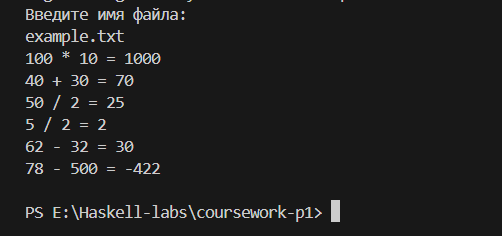
\includegraphics[width=0.6 \linewidth]{img/pic1.png}
	\caption{Результат работы программы.}
	\label{fig:pic1}
\end{figure}

Если какую-то строку разобрать невозможно, то программа выведет ошибку, последующие строки анализироваться не будут. Пример такого сценария показан на Рис.~\ref{fig:pic2}. Программа также выводит в консоль строку, которую не удалось разобрать.

\begin{figure}[H]
	\centering
	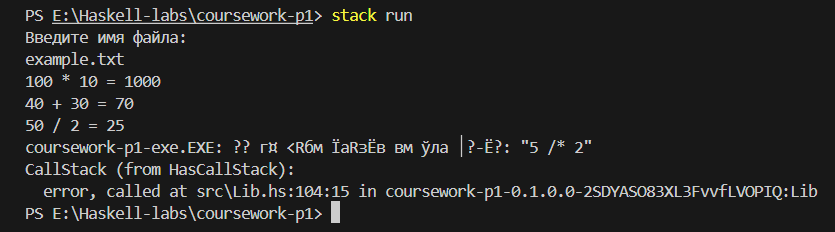
\includegraphics[width=0.8 \linewidth]{img/pic2.png}
	\caption{Результат работы программы.}
	\label{fig:pic2}
\end{figure}


Пример содержимого файла \texttt{expressions.txt} представлен ниже, в листинге ~\ref{lst:text}:

\begin{lstlisting}[caption={Код функции main}, label={lst:text}]
100 * 100
40 + 30
50 / 2
5 / 2
62 - 32
78 - 500
\end{lstlisting}

\subsection{Часть 2: Синтаксический анализ текста и генерация фраз}
Результаты работы программы представлены на Рис.~\ref{fig:pic3}. Программа предлагает пользователю ввести имя файла с текстом, а потом слово или пару слов, на основе которой генерируется и выводится ответ. Затем пользователю предлагается ввести имя ещё одного файла с текстом, задать начальное слово и размер диалога. После чего выводится диалог между полученными моделями, в скобках указано слово, с которого модель начала генерацию предложения.

\begin{figure}[H]
	\centering
	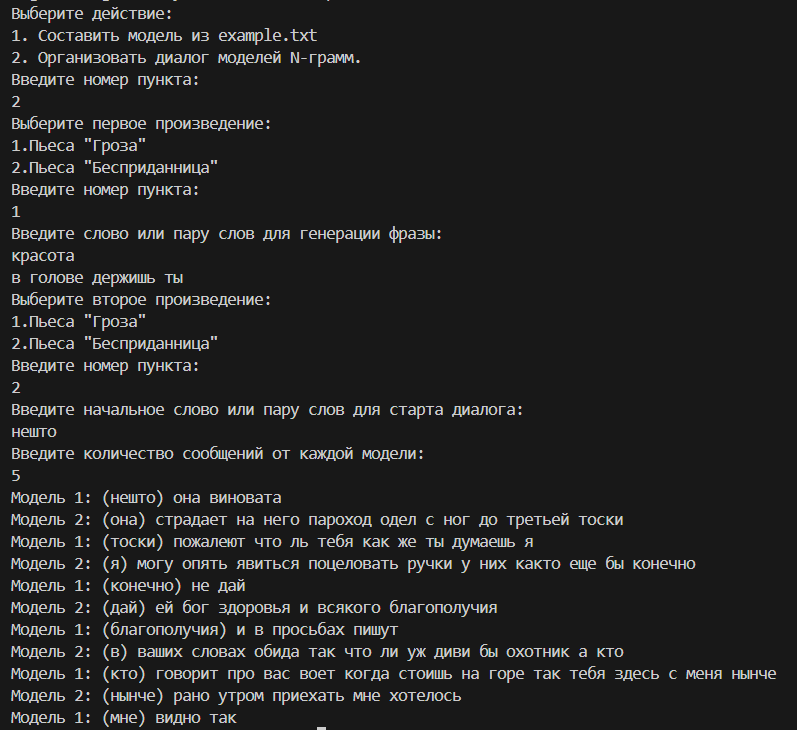
\includegraphics[width=0.8 \linewidth]{img/pic3.png}
	\caption{Результат работы программы.}
	\label{fig:pic3}
\end{figure}

Если заданного слова нет в словаре, то программа выводит сообщение об этом. По этой же причине диалог между моделями может прерваться преждевременно, о чём также будет сообщено пользователю. Пример такого сценария показан на Рис.~\ref{fig:pic4}.

\newpage
\begin{figure}[H]
	\centering
	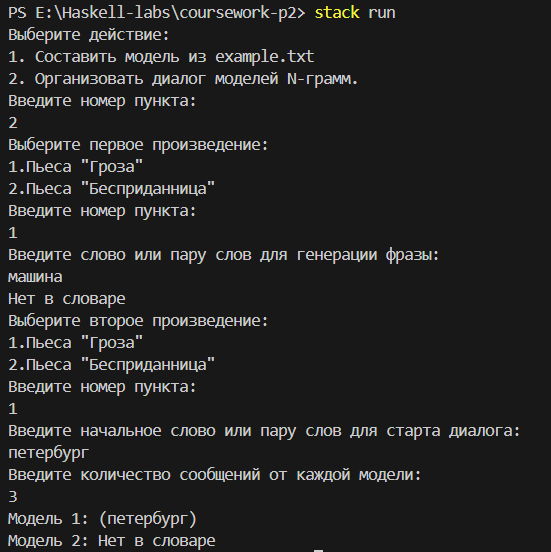
\includegraphics[width=0.8 \linewidth]{img/pic4.png}
	\caption{Результат работы программы.}
	\label{fig:pic4}
\end{figure}

Файлы \texttt{text1.txt} и \texttt{text2.txt} содержат пьесы Островского Александра Николаевича -- <<Гроза>> и <<Бесприданница>>. В первом тексте содержится 5869 слов, а во втором -- 5461. Первый абзац текста из файла \texttt{text1.txt} представлен ниже в листинге ~\ref{lst:text2}:

\begin{lstlisting}[caption={Текст произведения <<Гроза>>},stringstyle=\color{black},keywordstyle=\color{black}\bfseries]
ДЕЙСТВИЕ ПЕРВОЕ
Общественный сад на высоком берегу Волги, за Волгой сельский вид. 
На сцене две скамейки и несколько кустов.
ЯВЛЕНИЕ ПЕРВОЕ
Кулигин сидит на скамье и смотрит за реку. Кудряш и Шапкин прогуливаются.
Кулигин (поет). "Среди долины ровныя, на гладкой высоте..." '
(Перестает петь.) Чудеса, истинно надобно сказать, что чудеса! Кудряш! 
Вот, братец ты мой, пятьдесят лет я каждый день гляжу за Волгу и все 
наглядеться не могу.
Кудряш. А что?
Кулигин. Вид необыкновенный! Красота! Душа радуется.
Кудряш. Нешто!
Кулигин. Восторг! А ты "нешто"! Пригляделись вы либо не понимаете, какая 
красота в природе разлита.
\end{lstlisting}


Программа сохраняет словари N-грамм в файлы \texttt{dict1.txt} и \texttt{dict2.txt}. В результате запуска программы на текстах, описанных выше, файл \texttt{dict1.txt} содержит 4642 строк, а файл \texttt{dict2.txt} -- 4477. Каждая строка файла представляет собой ключ и значение из словаря. Ключ это одна из N-грамм, а значение это список N-грамм, которые являются возможными продолжениями текста. Первые десять строк содержимого файла \texttt{dict1.txt} представлены ниже:

\begin{lstlisting}[caption={Первые 10 N-грамм из словарь произведения <<Гроза>>},stringstyle=\color{black},keywordstyle=\color{black}\bfseries]
"а": ["ты нешто","п к","этот как","то бы","что бы","про нашу","я с","пущай же","я десять","то что","сестру в","кончит всетаки","то сестру","жалованья что","может я","уж где","уж пуще","беда как","потом и","вот бедато","каково домашнимто","всетаки не","у кого","между собойто","те им","там уж","они еще","вы умеете","ведь тоже","тоже есть","особенно дому","домашних заела","то руки","работать нечего","вы надеетесь","мне видно","тут еще","как ты","вы молодые","это нынче","сохрани господи","так к","может и","к родительнице","ты еще","б а","н о","теперь поедом","еще говоришь","то маменька","то знаешь","придем из","странницы станут","я по","вечером опять","то бывало","какие сны","как на","то будто","что же","вот что","удержаться мне","то нехорошо","на уме","точно меня","ты почем","вот погоди","что за","коли далеко","право бы","как я","что хозяйкато","вы девушка","вы все","к нам","я милая","ты феклуша","слыхать много","салтаны землей","в другой","у них","поихнему все","то есть","мы тут","дело было","парни поглядывали","ведь ты","ведь без","ты меня","сама напоминаешь","он так","не стерпится","уж коли","мне нужно","то неужто","т е","сам думает","потом приедешь","что","ты","п","этот","то","про","я","пущай","сестру","кончит","жалованья","может","уж","беда","потом","вот","каково","всетаки","у","между","те","там","они","вы","ведь","тоже","особенно","домашних","работать","мне","тут","как","это","сохрани","так","к","б","н","теперь","еще","придем","странницы","вечером","знаешь","какие","удержаться","на","точно","коли","право","слыхать","салтаны","в","поихнему","мы","дело","парни","сама","он","помоему","не","т","сам"]
"а б": ["а"]
"а беда": ["как"]
"а в": ["другой"]
"а ведь": ["тоже","ты","без"]
"а вечером": ["опять"]
"а вот": ["бедато","что","погоди"]
"а всетаки": ["не"]
"а вы": ["умеете","надеетесь","молодые","девушка","все"]
"а дело": ["было"]
\end{lstlisting}



\newpage
\section*{Заключение}
\addcontentsline{toc}{section}{Заключение}
В рамках курсовой работы были разработаны и реализованы два \texttt{stack} проекта на языке Haskell, соответствующих поставленным задачам. 

Первый проект представляет собой синтаксический анализатор для обработки строк, содержащих целые числа и бинарные операции. Реализация включала чтение данных из файла, синтаксический разбор выражений и вычисление их результатов.

Второй проект — синтаксический анализатор текста и генератор продолжения текста, основанный на модели N-грамм. Проект включает функционал по синтаксическому разбору текста, удалению пунктуации и цифр, построению словаря биграмм и триграмм, генерации текста, а также ведению диалога между моделями, созданными на основе двух разных текстов. Для демонстрации работы программы были взяты два произведения А.Н. Островского: «Гроза» (5869 слов) и «Беприданница» (5461 слова).

В ходе работы были выполнены все поставленные задачи, а полученные знания могут быть использованы в других проектах на языке Haskell.


\newpage
\section*{Список литературы}
\addcontentsline{toc}{section}{Список литературы}

[1] Hackage -- unescaping-print: Tiny package providing unescaping versions of show and print, URL: \url{https://hackage.haskell.org/package/unescaping-print}, Дата обращения: 15.12.2024.


\end{document}